\chapter[宇佐见堇子的 \LaTeX 之旅]{宇佐见堇子的 \LaTeX 之旅}
\label{cp:宇佐见堇子的 LaTeX 之旅}
\addauthor{小飞舞}
\begin{center}
    \begin{tcolorbox}[colback=black!15!white,%gray background
            colframe=black!80,% black frame colour
            width=15cm,% Use 5cm total width,
            arc=2mm, auto outer arc,
            boxrule=0.5pt,
            title=前言,
            fontupper = \itshape,
            % code before = {\setlength{\parindent}{2em}}
        ]
        话说那宇佐见堇子考入了东京大学第一年就做出了相当成功的研究,正在她想把自己的想法发表在网络上的时候,她犹豫了。

        用什么组织自己的文章呢?她想。在东深见高中上学的时候,自己就曾经用 Blog 的形式将幻想乡的一些讯息扩散出去——虽然总是被当成都市传说,但也是的的确确可以在自己的电脑上随意部署样式。但现在不一样了,既然是专业性的论文,那在自己的 Blog 上部署也太看不起自己了——好歹要传到专业性的期刊上去!要不然实在太枉费自己了。

        \url{http://arxiv.org/}

        这样一个网站,上面收集了很多关于物理、数学。计算机科学等学科的论文。虽然看上去平平无奇,但的确有些非常厉害的数学家在上面发表极具影响力作品的历史\footnote{比如格里戈里·雅柯夫列维奇·佩雷尔曼 (Grigori Yakovlevich Perelman) 在 2002 年 11 月发表的解决几何化猜想 (Geometrization conjecture) 的论文。}。她当即决定就这个了。不过她在查找资料的时候注意到了要是用 \TeX 格式发表自己论文的事情,这让她非常疑惑——不是只要写出来就行吗?还管那么多格式干嘛?

        于是她找到了同样在东京大学任副教授的宇佐见莲子……
    \end{tcolorbox}
\end{center}


“呃……当时也差不多就是在那种情况下学习 \LaTeX 的,不过我倒觉得这玩意蛮重要的。”宇佐见莲子对面前的年轻学生说道。“后来……由于工作的需要,需要使用 \LaTeX 的方面也变多了——其实不只是像我这样的物理人,我觉得只要是理科都有可能会接触到 \LaTeX 的。”

“啊其实就是说……这玩意看上去高级,但是听说不太好学,呃……”上了大学后,宇佐见堇子明显稳重了许多,也不再穿她那非主流的服装了。此时她看起来和正常的学生毫无二致。

除了她在大一就已经有了成果之外。

“其实并不是这样……大多数人一开始学 \LaTeX 是为了排版自己的论文,如果只是做到这样的话学习并不算难……当然你也可以用她来排版些奇奇怪怪的东西。”宇佐见莲子说道,她轻轻撩了撩头发,“反正现在时间还早,我就先说说关于 \LaTeX 有趣的事情吧。”

“啊?你不帮我排版吗?”

“自己排啦~反正学会这个之后也是有利无害。”

\section{什么是 \LaTeX}

“\TeX 是高德纳 (Donald E. Knuth) 为排版文字和数学公式而开发的软件。当时他正在想办法出版他的巨作《计算机程序设计艺术》的前三卷,但作为“艺术”类的作品,高德纳实在无法忍受当时的排版质量——那时是 1977 年,与我们现在相差非常大的年份。\TeX 大约在 1989 年开发到一个在当时比较完善的地位,然后—— Leslie Lamport 博士在此基础上开发了 \LaTeX,实际上就是一组用 \TeX 语言的宏,那时候就大概是上世纪八十年代处左右吧。”

“那时候的人们都那么勇吗?为了排版直接写引擎?”宇佐见堇子脸上写满了惊讶。

“你要知道《计算机程序设计艺术》是多么宏伟的巨作——这玩意花费了高德纳将近一生的时光,直到现在还没写完。”宇佐见莲子摆起认真相。

“\LaTeX 相比 \TeX 有很多优势——比如在 1994 年后,\LaTeXe{} 已经完善,这玩意已经逐步称为国际上排版数学、物理、计算机等科技领域专业出版物的标准。而 \LaTeX 比 \TeX 本身更容易使用——高德纳开发 \TeX 本质是只为了自己的鸿篇巨制,而 \LaTeX 在此基础上定义了一些宏和格式,其实就将部分排版细节隐藏起来,相对而言更容易点——对你这种只想排论文的再好不过了。当然,你也可以拿 \LaTeX 来写笔记,看起来会比手写的要美观很多……一言以蔽之:


\begin{itemize}
    \item \LaTeX 具有专业的排版输出能力,本身就是为了美观而服务的。
    \item \LaTeX 目前仍是最强大的公式排版系统之一。
    \item 这玩意可以让用户更专注与内容、而不是被错综复杂的版式耍的团团转。
    \item 有很多面向 \LaTeX 开发的宏包可以解决各式各样的问题。
    \item 横跨全平台,而且开源免费。
\end{itemize}

“看起来感觉还不错。”宇佐见堇子舔了舔嘴唇。

“我们先从看得见的地方开始说起吧:首先就是这玩意的下载以及安装。”

\subsection{\LaTeX 的下载与安装}

\LaTeX 有很多发行版,比如 \verb"TeXlive", \verb"MiKTeX", \verb"MacTeX" 这些,每个发行版可能有不同的宏包管理器( \LaTeX 很多实现都是要依赖宏包才比较好搞),在这里我推荐的是比较全的 \verb"TeXlive" ,因为我用的就是 \verb"TeXlive" ,所以以下的教程全部以 \verb"TeXlive" 为基准。同样的,以下的教程基于 Windows 10。

我们仅仅需要打开 \verb"TeXlive" 的相关网站 \link{https://tug.org/texlive/},然后选择

\begin{center}
    \vbox{\textbf{\sffamily All the ways to acquire TeX Live:} $\longrightarrow$ {\sffamily on DVD}

        $\longrightarrow$ {\sffamily downloading the TeX Live ISO image and burning your own DVD}

        $\longrightarrow$ {\sffamily download from a nearby CTAN mirror}}
\end{center}

然后下载 \verb"texlive2022.iso"\footnote{根据年份不同可能会发生改变。} 即可。当然如果嫌慢,也可以使用一些镜像源:

\begin{itemize}
    \item \url{https://mirrors.nju.edu.cn/CTAN/systems/texlive/Images/}
    \item \url{https://mirrors.tuna.tsinghua.edu.cn/CTAN/systems/texlive/Images/}
    \item \url{https://mirrors.aliyun.com/CTAN/systems/texlive/Images/}
    \item \url{https://mirrors.sjtug.sjtu.edu.cn/ctan/systems/texlive/Images/}
\end{itemize}

反正各大学校一般都会有自己的镜像源,一样下载即可。

下载完成后可以运行 \verb"install-tl-windows.bat" 进行安装,选项默认就行,静待安装完成。

“呃……这个 ISO 文件怎么处理啊?”宇佐见堇子挠了挠头。

“直接解压就行了,里面就有一个 \verb"install-tl-windows.bat"。”

``什么? 你说你用的是Mac啊\dots

那就更方便了。

我们仅仅需要打开 \verb"MacTeX" 的相关网站 \link{https://tug.org/mactex/index.html},然后选择

\begin{center} \vbox{\textbf{\sffamily MacTeX Download}
$\longrightarrow$ {\sffamily MacTeX.pkg}
\end{center}

现在应该已经开始下载了。

下载完成后双击安装就行。''



\subsection{\LaTeX 的初步使用}

“安装完你的电脑里就有这么一个叫做 \LaTeX 的东西了,然后打开你的 Windows 菜单,应该会有一个 \verb"TeX live" 文件夹,里面有一个 \verb"TeXworks editor" 的软件,这是 \verb"TeXlive" 自带的一个 \LaTeX 代码编辑器。

如果是Mac,按下键盘上的F4进入启动台。你可以在里面找到一个名字叫 \verb"TeX" 的文件夹,里面有一个 \verb"TeXShop" 的软件。同样地,这也是 \verb"MacTeX" 自带的一个 \LaTeX 代码编辑器。

在里面可以写代码:

\begin{lstlisting}
    \documentclass{article}
    \begin{document}
    The quick brown fox jumps over the lazy dog.
    % use '%' to set single-line comments
    \end{document}
\end{lstlisting}

然后在左上角复选框(Mac是窗口的上部)里面选择你要使用的引擎:

\begin{itemize}\ttfamily
    \item pdfTeX
    \item pdfLaTeX
    \item XeTeX
    \item XeLaTeX
    \item \dots
\end{itemize}

这些玩意各有千秋,给我的感觉大概是这样子的:

\begin{itemize}
    \item \verb"pdfLaTeX"
          \begin{itemize}
              \item 古老
              \item 编译很快
              \item 不原生支持 Unicode,这意味着如果你要写中文的话会很麻烦,而且如果你想要哪怕是一点点花里胡哨的视觉效果都最好别用 \verb"pdfLaTeX"。
          \end{itemize}
    \item \verb"XeLaTeX"
          \begin{itemize}
              \item 比较现代
              \item 编译有点慢
              \item 原生支持 Unicode
              \item 有一些宏包是只支持 \verb"XeLaTeX" 和 \verb"LuaLaTeX" 的,比如 \verb"Unicode-math" 宏包(但“支持”是相对 \verb"pdfLaTeX" 来说的)
          \end{itemize}
    \item \verb"LuaLaTeX"
          \begin{itemize}
              \item 允许写 Lua 代码来拓展功能
          \end{itemize}
\end{itemize}

这边咱呢会选择 \verb`XeLaTeX`,这个比较常用——我们的目的是要有 CJK\footnote{CJK文字是中文、日文和韩文的统称} 支持。”

“CJK?就是中日韩吧?这不支持 Unicode 的特点也太烦人了……”宇佐见堇子喃喃道。

“那时候还没有 Unicode 啊!”莲子大叫道。

保存后编译不出意外的话打开个 PDF 预览器,结果正如 \autoref{fig:lazyDOG} 所示。

\begin{figure}[t]
    \centering
    \begin{subfigure}[t]{0.4\textwidth} \centering
        \boxed{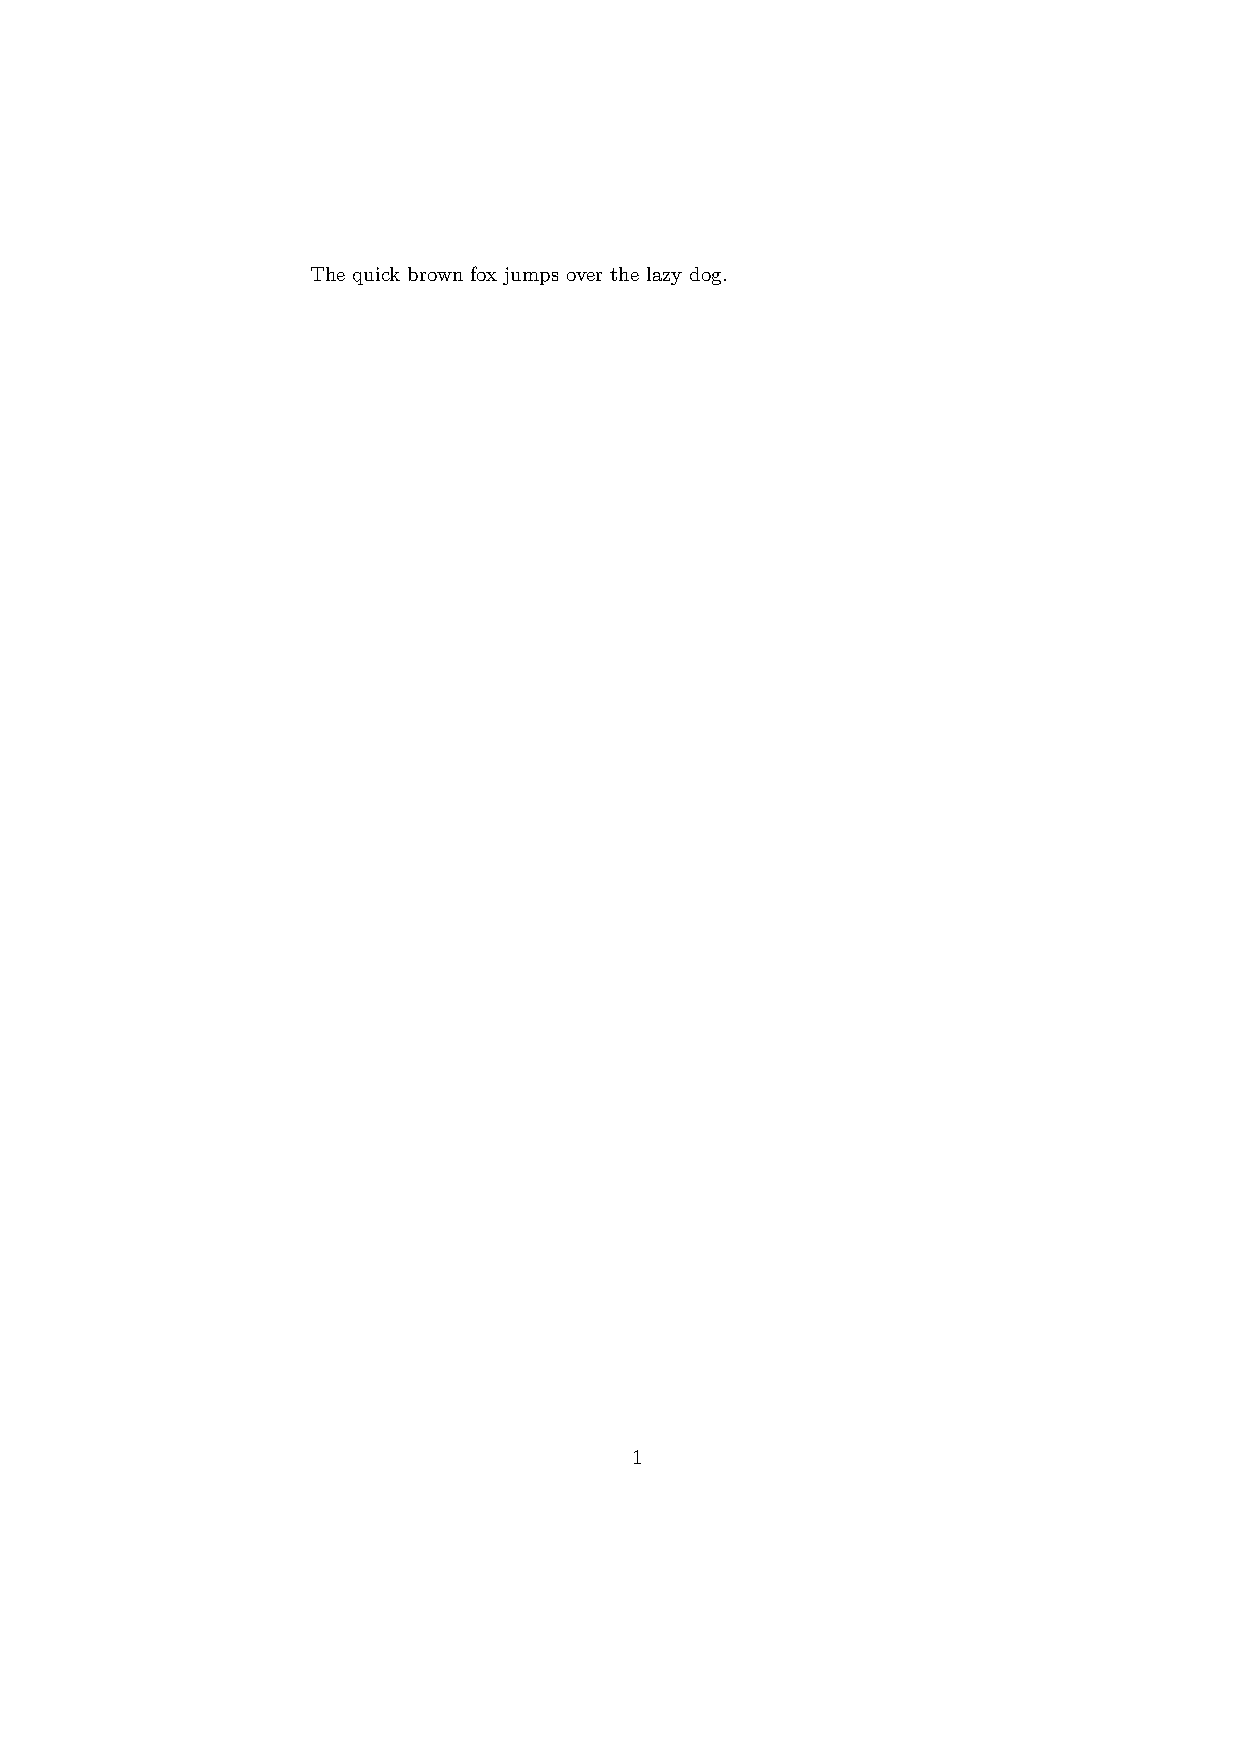
\includegraphics[width = \textwidth]{lazydog.pdf}}
        \caption{第一次编译}
        \label{fig:lazyDOG}
    \end{subfigure}\quad
    \begin{subfigure}[t]{0.4\textwidth} \centering
        \boxed{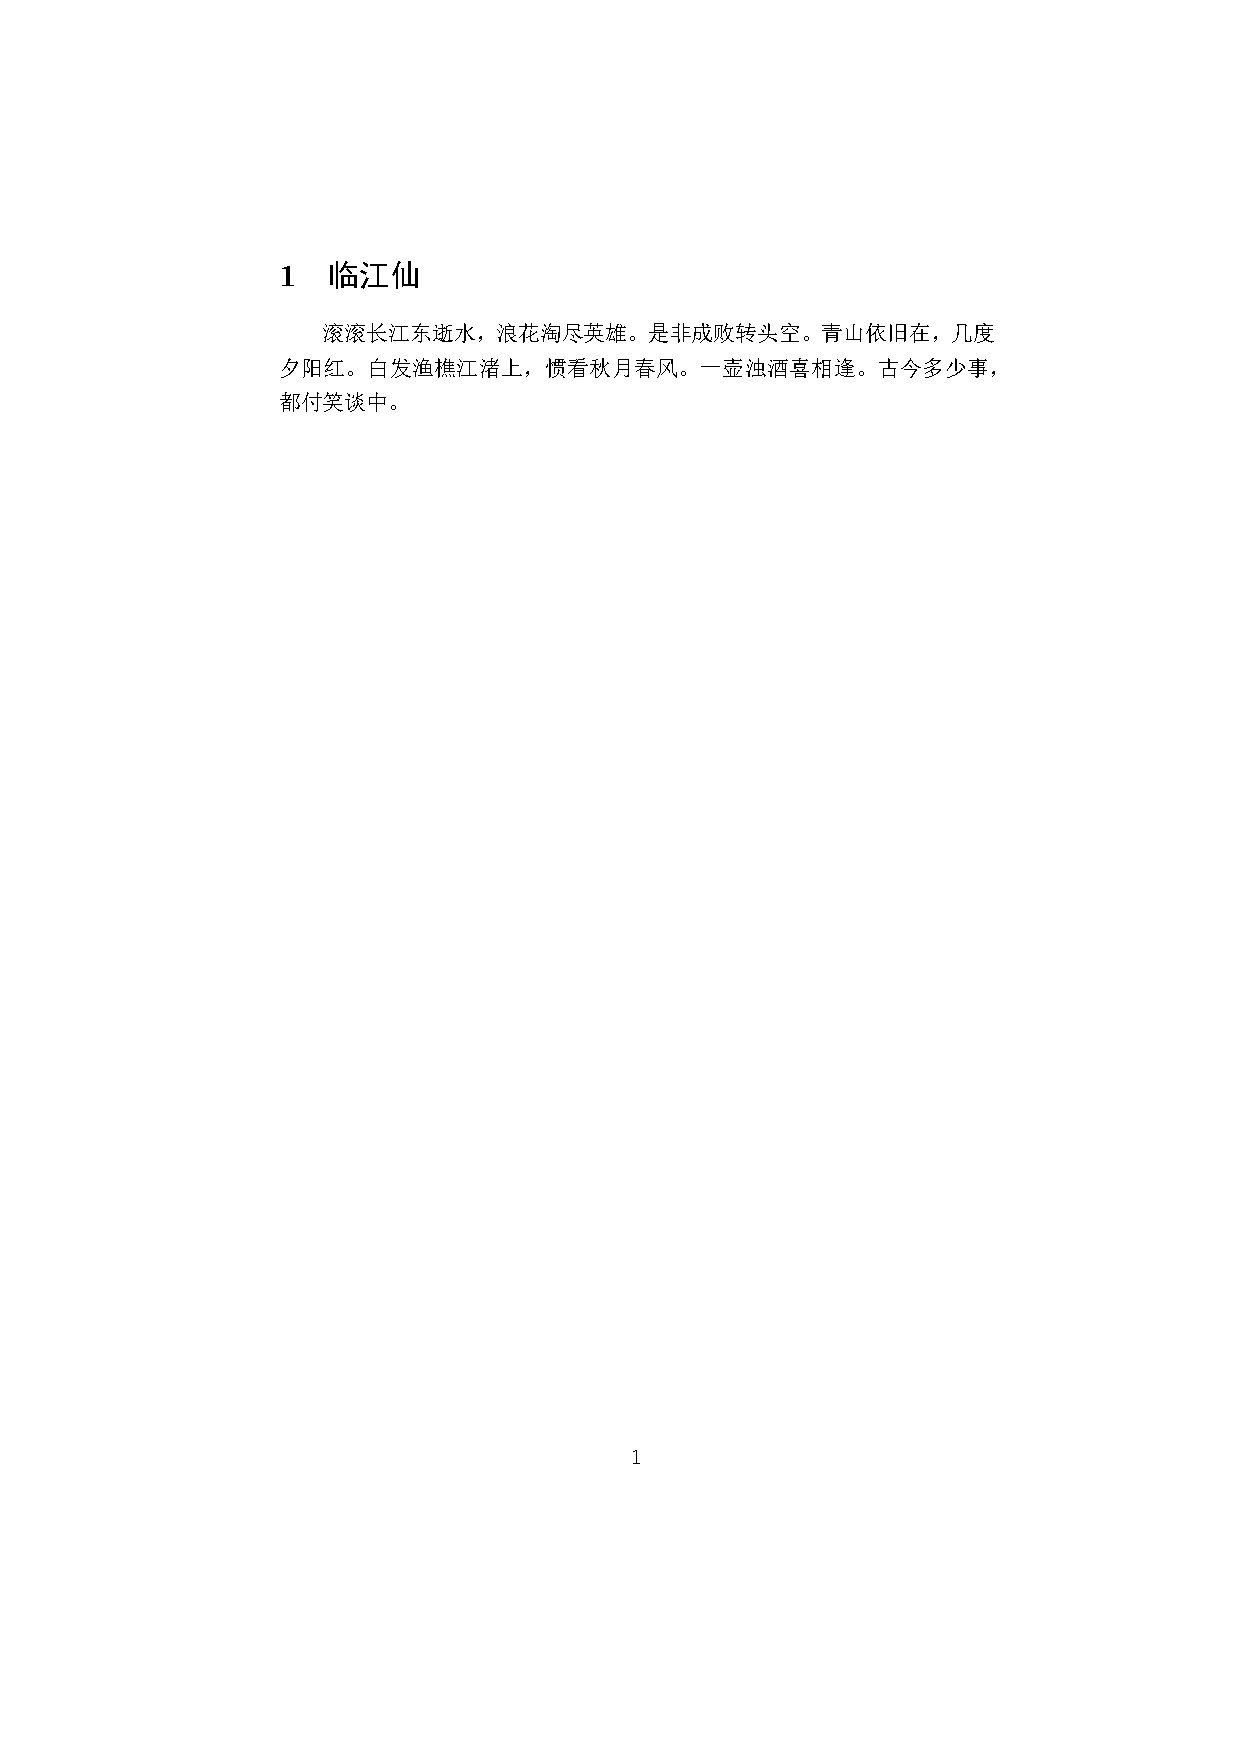
\includegraphics[width = \textwidth]{ggcjdss.pdf}}
        \caption{一个带中文的例子}
        \label{fig:滚滚长江东逝水}
    \end{subfigure}
\end{figure}

接下来写些带其他文字的例子 \autoref{fig:滚滚长江东逝水} :


\begin{lstlisting}
    \documentclass{article}
    \usepackage{ctex}
    \begin{document}
    \section{临江仙}
        滚滚长江东逝水,浪花淘尽英雄。是非成败转头空。
        青山依旧在,几度夕阳红。

        白发渔樵江渚上,惯看秋月春风。一壶浊酒喜相逢。
        古今多少事,都付笑谈中。    
    \end{document}
\end{lstlisting}


“我来解释一下这里面的命令……

\begin{itemize}
    \item \verb"\documentclass{article}" 指的是使用 \verb"article" 文档类,这意味着还有其他的文档类,比如说 \verb"book"、\verb"ctexart" 这些。
    \item \verb"\usepackage{ctex}" 是在这里引用了一个叫做 \verb"ctex" 的宏包,这个宏包正是用来处理 CJK 字符的。
    \item \verb"\begin{document}" 和 \verb"\end{document}" 之间就是咱们的正文区了,在此之前就是引言区(主要来作一些全局设置的)。
\end{itemize}

不过值得注意的是,代码的换行并不会引起 PDF 内内容的分段,至少需要连续换两行才行。”

“这看起来倒像是合乎常理的……毕竟代码不能一行写太长嘛……”

“其实倒也不是这样,因为 \LaTeX 里面的换行其实有点像空格……在某些层面影响很大的。”莲子纠正道,“我给你看个好康的例子。”


\begin{lstlisting}
    \documentclass{article}
    \usepackage{ctex}
    \begin{document}
        \colorbox{red}{
            \color{white} 
            A spanning list in a vector space may not be a basis because it is not linearly independent.
        }
    \end{document}
\end{lstlisting}

\begin{center}\footnotesize
    \colorbox{red}{
        \color{white}
        A spanning list in a vector space may not be a basis because it is not linearly independent.
    }
\end{center}

“看起来好像没啥,实际上——A 前面是有一个空格的,这个空格实际上是来自于代码换行。”

“哦哦!所以我是不能随便换行的对吧,那这样太离奇了吧?写代码不能随便换行??”

“呃……其实有方法可以规避的……我们一般会在折行处加一个 \verb"%" 符号,这样子就可以注释掉后面的换行(空格)了。”


\begin{lstlisting}
    \colorbox{red}{%
        \color{white}%
        A spanning list in a vector space may not be a basis because it is not linearly independent.%
    }
\end{lstlisting}

\begin{center}\footnotesize
    \colorbox{red}{%
        \color{white}%
        A spanning list in a vector space may not be a basis because it is not linearly independent.%
    }
\end{center}

“呒呒呒,原来注释还有这种用法。”堇子挠了挠头,“我还是第一次见。”

“以后有得你见的,有关 \LaTeX,有趣的事情不少。这种注释也只用在你想写一些正经代码的时候。”

\subsection{用 \LaTeX 组织你的文档——最初的例子}

“行了,说了那么多废话,我们来看看一个带数学公式的例子。”

“哦这么说差点忘了,之前一直在听你说故事什么的,原本自己想干什么都忘了。”

“公式嘛……其实与正文不一样,因此要提供一个‘数学环境’这样的东西。”


\begin{lstlisting}
    \documentclass{article}
    \begin{document}
        as we know:
        \[
            \sum_{n=0}^\infty \frac{1}{n!} = \exp (1)
        .\]
        and $\sin \left( \frac{\pi}{2} \right) = 1 $.
    \end{document}
\end{lstlisting}

得到 \autoref{fig:firstmath}。

\begin{figure}[th]
    \centering
    \boxed{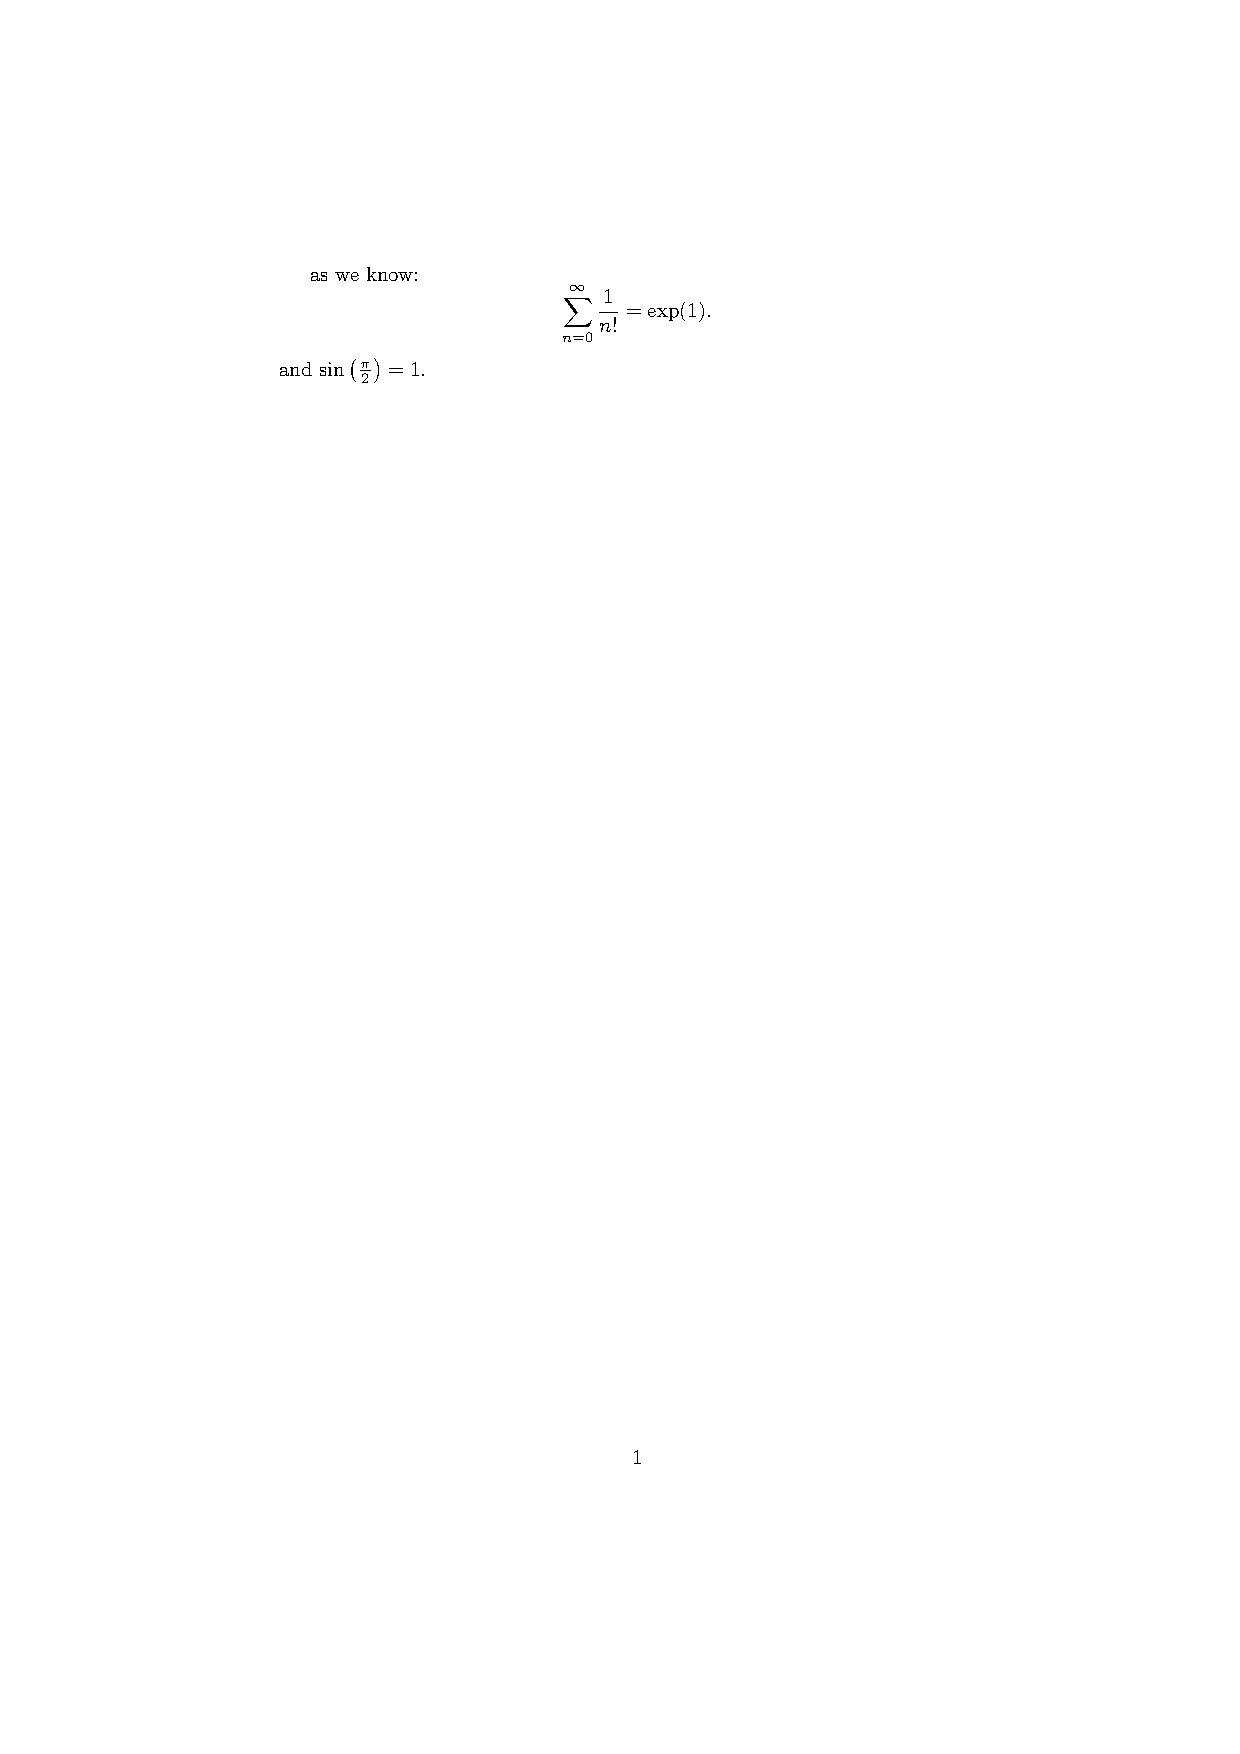
\includegraphics[width = 0.4 \textwidth]{first math ex.pdf}}
    \caption{一个带了数学环境的例子}
    \label{fig:firstmath}
\end{figure}


其中我们会认为:
\begin{itemize}
    \item \verb"\[...\]" 之间是\textbf{行间公式}环境,我们可以称为``displaystyle math''。
    \item 与之对应的,\verb"$...$" 是行内数学公式环境,可以称为``textstyle math''。
\end{itemize}

当然以上两种也可以用 \verb"$$...$$" 和 \verb"\(...\)" 来代替,虽然我不推荐\footnote{\texttt{\char"005C[...\char"005C]} 比 \texttt{\$\$...\$\$} 多了一层检查用于 \texttt{\char"005C @badmath} 报错,且还支持一些选项(比如说公式左对齐的 \texttt{fleqn} 选项、 \Verb{\tag} 命令等)而 \texttt{\char"005C(...\char"005C)} 则不是 Robust 的命令,具体见 \textcite[The \LaTeXe{} Sources]{braams2003latex2varepsilon} \link{https://www.ctan.org/pkg/source2e}。}就是了。在例子中可以很清楚对照到“上标”是 \verb"^{...}",下标是 \verb"_{...}" ,当只有一个字符的时候可以省略掉大括号。 至于像其他乱七八糟的数学符号命令现在在这里全部说明也不适合——具体可以参考——呃算了等到一会我回去的时候给你些链接。”

“链接?不会又是什么全英文地狱电子文档吧?”堇子试探性的问道。

“有些还是有翻译的。”莲子认真地说道,“总之我们继续。”

“在除去数学公式这一巨大的板块后, \LaTeX 当然可以参与普通的排版,在 \verb"article" 类中有很多章节层级,按以下顺序排列:

\begin{center}
    \begin{tblr}{cll}
        \hline
        层次 & 命令                              & 说明                                \\\hline
        $-1$ & \ttfamily\char"005C part          &                                     \\
        $0$  & \ttfamily\char"005C chapter       & \texttt{article} 类中并没有这个章节 \\
        $1$  & \ttfamily\char"005C section       &                                     \\
        $2$  & \ttfamily\char"005C subsection    &                                     \\
        $3$  & \ttfamily\char"005C subsubsection & 默认不编号、不编目录                \\
        $4$  & \ttfamily\char"005C paragraph     & 同上                                \\
        $5$  & \ttfamily\char"005C subparagraph  & 同上                                \\\hline
    \end{tblr}
\end{center}

在此机制之上我们就可以组织我们文档的层级了。”


\begin{lstlisting}
    \part{Algebra}
    \section{Groups}
    \subsection{Free groups}
    \paragraph{The constrution of free groups}
        We know $A$ is just a...
\end{lstlisting}



\begin{tcolorbox}[sharp corners]
    {\noindent\Large\bfseries Part\nobreakspace I
        \par\nobreak
        \noindent{\huge \bfseries Algebra%
            \par}\nobreak
        \vskip 2ex}
    {\noindent\Large\bfseries 1\kern2.3ex Groups}

    \vskip3.25ex\noindent{\normalfont\large\bfseries 1.1\kern2.25ex {Free groups}}\vskip1.3ex

    \paragraph{The constrution of free groups}
    We know $A$ is just a...
\end{tcolorbox}



“感觉不如 \verb"markdown"%\simpleicon{markdown}}
方便。”堇子吐槽道。

“请注意你的言辞,难道你要用 \verb"markdown" 写论文吗?”莲子正色道,“这玩意不保真啊。”

“可是我用 \verb"CSS" 也可以仿出这样的标题形状哇。”堇子反驳道。“ \verb"markdown"%\simpleicon{markdown}} 
写得多轻巧,这 \LaTeX 写之前我还要安装个 4 GiB 的大家伙。”

“好,你用 \verb"CSS" 写个正经的折行分页算法给我看看吧。”莲子面无表情地说道。

堇子不吱声了。



\section{\LaTeX 与数学排版}

“首先先说一点前置的东西——数学公式,如你所见,有上标、下标。因此是「二维」的,必然不可能仅仅靠字偶距\footnote{一般称为 kerning,一般字体在某些字母字面框对齐的情况下会显得比较难看: {Y}{a} 和 Ya 分别是在 Y 和 a 中间有无插入微小负间距的对比。}来微调,还要依靠上下的移动来达到比较好的效果——这显然是相当麻烦的。因此不要在数学环境里玩花。”

“草,这感觉要把这所见非所得的东西玩出所见即所得的形状出来。”

“我们应该知道一些规范,比如说正儿八经的公式就应该用正儿八经的数学环境:

“a - b 和 $a - b$,就分别是正文环境与数学环境的例子。因为在前者中 \verb"-" 是作为连字符呈现的,而后者是正儿八经的「减号」。正如前面展示的数学例子一样,我们用 \verb"$...$" 和 \verb"\[...\]" 来声明数学环境。”

\subsection{\AmS 与一些规范}

“进入数学环境之后,我们就不允许像在正文环境那样随意了,首先是一个痛点——在数学环境尽量避免使用非 ASCII\footnote{即
    American Standard Code for Information Interchange,你可以认为是美式键盘上可以直接输入的所有字符。} 代码,否则——:

“\verb"$A^ {ij} _{γ}$" 会得到$
    A^{ij} %_{γ}
$,这样子 $\gamma $ 显然没办法正常显示\footnote{除非你引入可以在数学环境进行特殊处理的包,比如 \texttt{unicode-math}.},如果要打出正常的希腊字母 $\gamma $只需打出 \verb"\gamma" 即可,其他希腊字母照常。

“草草,这也太离谱了,什么都不让用。”

“本身代码这种就最好纯用 ASCII 写啊,况且你不想想那是什么年代。另外还有一些事情是要注意的,那就是要按照正常的科技规范来正确输入,我们引入 \AmS{}Math 这个数学宏包——


\begin{lstlisting}
    % \usepackage{amsmath}
    \[
        \sum_{n=0}^{\infty} \frac{x^n}{n!} = \mathrm{e} ^ x
    .\]
\end{lstlisting}

自然就会得到:



\[
    \sum_{n=0}^{\infty} \frac{x^n}{n!} = \mathrm{e} ^ x
    .\]
“长得挺好看的这公式。”堇子立刻评论道。

“对,你看这个里面有这么一个命令 \verb"\mathrm",这玩意是将吸收的参数转化为 roman 字形,在科技文献中我们会一般要求自然对数的底 $\mathrm{e}$ 要正体,同理,面对虚数单位 $\mathrm{i}$,微分算子 $\mathrm{d}$ 也最后如此:
\[
    \int_0^{2\symup\pi } \mathrm{e} ^ {2 \mathrm{i} z } \,\mathrm{d}z = 0
    .\]
当然你不这么写也行,但这样看上去比较好看。

另外一个,一些函数的名字是可以用反斜杠加上函数名打出来的:

\begin{center}
    \begin{tabular}{cc}
        \verb"\sin z" & $\sin z$ \\
        \verb"sin z"  & $sin z$  \\
    \end{tabular}
\end{center}

“草我在一些论坛上面逛的就看到后面这种,难看死了。”

“对,而且也不合规范——这一点如果不熟悉的话还是要注意的。归根到底,其实是 \verb"\sin" 本身就是一个新的命令,展开后会得到正体的 $\sin $ 以及和后面的变量之间\textbf{带上空格}\footnote{其实不应该叫空格,叫glue更恰当。}。可以看到在上面的例子中,即使在代码里面加入空格,真正显示出来的也不会有空格。

“草这空格怎么那么麻烦……”

“先不管,我们看看这个神奇妙妙——\footnote{下面的「代码」默认在数学环境里,因此不加数学环境的声明了,此处参考 \textcite[Symbols defined by unicode-math]{WillRobertson} \link{https://mirrors.nju.edu.cn/CTAN/macros/unicodetex/latex/unicode-math/unimath-symb}。}:

\begin{table}[h]
    \centering
    \caption{一些数学字符的近似分类}
    \DefTblrTemplate{caption-tag}{default}{}
    \DefTblrTemplate{caption-sep}{default}{}
    \begin{tblr}{colspec = {X[-1]XX[-1]}, width = \textwidth}\hline
        分类                 & 代码                                                                                                                         & 预览                                                          \\\hline
        Opening symbols      & \texttt{\char"005C (, [, \char"005C\{, \char"005Clceil, \char"005Csqrt\{\}}                                                  & $(,~[,~\{,~\lceil,~\sqrt{}$                                   \\
        Closing symbols      & \texttt{\char"005C !, ), ], \char"005C\}, \char"005C rfloor}                                                                 & $!,~),~],~\},~\rfloor$                                        \\
        Fence symbols        & \texttt{\char"005C | = \char"005C vert, \char"005C Vert = \char"005C|}                                                       & $| = \vert,~\Vert~= \|$                                       \\
        Punctuation symbols  & \texttt{\char"005C , : ;}                                                                                                    & $, : ;$                                                       \\
        Over symbols         & \texttt{\char"005C overbrace\{a + b\}\^{}M}                                                                                  & $\overbrace{a + b}^M$                                         \\
        Under symbols        & \texttt{\char"005C underbrace\{h + k\}\_L}                                                                                   & $\underbrace{h + k}_L$                                        \\
        Accents              & \texttt{\char"005C bar\{x\}, \char"005C tilde\{x\}, \char"005C dot\{x\}, \char"005C ddot\{x\}, \char"005C mathcirc\{x\}}     & $\bar{x},~\tilde{x},~\dot{x},~\ddot{x},~\mathring{x}$         \\
        Math operators       & \texttt{\char"005C sin, \char"005C lim, \char"005C inf}                                                                      & $\sin,~\lim,~\inf$                                            \\
        BIG Math operators   & \texttt{\char"005C int\_0\^{}1 \char"005C sum\_0\^{}1 \char"005C displaystyle \char"005C int\_0\^{}1 \char"005C sum\_0\^{}1} & $\textstyle\int_0^1 \sum_0^1 \displaystyle \int_0^1 \sum_0^1$ \\
        Binary relations     & \texttt{\char"005C a+b, a\{+b\}, - ,\char"005C times, \char"005C div}                                                        & $a + b,~a{+b},~- ,\times,~\div$                               \\
        Ordinary symbols     & \texttt{\char"005C forall, \char"005C exists, \char"005C emptyset}                                                           & $\forall,~\exists,~\emptyset$                                 \\
        Relation symbols     & \texttt{\char"005C a<b, a\{<b\}, \char"005C to, \char"005C leftarrow, \char"005C mapsto}                                     & $a<b,~a{<b},~\to,~\leftarrow,~\mapsto$                        \\
        Alphabetical symbols & \texttt{\char"005C pi, \char"005C mathbf\{A\}, \char"005C mathcal\{X\}, \char"005C mathsf\{C\}}                              & $\pi,~\mathbf{A},~\mathcal{X},~\mathsf{C}$                    \\\hline
    \end{tblr}
\end{table}

“草这也太哈人了吧。”堇子大叫道。

“呃……实际上也只是展示出来而已,就是个分类,我们在里面可以看到一些有趣的细节……比如说 Binary relations 只有在前后两个都是其他数学符号的时候,两边才会安插一个空格——与 Relation symbols 的表现明显不一样,逗号和冒号都是正儿八经的标点符号,但逗号后面会有被动的空格,巨算符 (BIG Math operators) 在行间公式和行内公式形状不同等等,都是非常细节的东西。”

“哇,好~厉~害~哦!请问这些细节有什么用捏?”

“草……只是说无论你知晓与否,的确是有很多细节在里面的……这样可以让你对其保持敬畏。”
\subsection{字体与数学字体}

“在排版中,我们当然不会只用一种字体,而是使用各种各样形状的——见 \autoref{tab:字形们}\footnote{此处使用字体为:  宋体:Noto Serif CJK SC;黑体:Noto Sans CJK SC;楷体:方正楷体;西文衬线体:\TeX{} Gyre Pagella;西文无衬线体:Noto Sans;等宽字体:Iosevka。}。且不同的性质 \verb"shape", \verb"family", \verb"series" 可以叠加。”

“啦特可爱是什么意思?”堇子问道。

\begin{table}[h]
    \centering
    \caption{控制字形的主要三组参数}
    \begin{tblr}{l|l|l}
        \hline
        \Verb{{\mdseries ABCabc123啦特可爱}} & \Verb{\textup{ABCabc123啦特可爱}} & \mdseries ABCabc123啦特可爱 \\
        \Verb{{\bfseries ABCabc123啦特可爱}} & \Verb{\textbf{ABCabc123啦特可爱}} & \bfseries ABCabc123啦特可爱 \\
        \hline
        \Verb{{\itshape ABCabc123啦特可爱}}  & \Verb{\textit{ABCabc123啦特可爱}} & \itshape ABCabc123啦特可爱  \\
        \Verb{{\slshape ABCabc123啦特可爱}}  & \Verb{\textsl{ABCabc123啦特可爱}} & \slshape ABCabc123啦特可爱  \\
        \Verb{{\scshape ABCabc123啦特可爱}}  & \Verb{\textsc{ABCabc123啦特可爱}} & \scshape ABCabc123啦特可爱  \\
        \hline
        \Verb{{\rmfamily ABCabc123啦特可爱}} & \Verb{\textrm{ABCabc123啦特可爱}} & \rmfamily ABCabc123啦特可爱 \\
        \Verb{{\sffamily ABCabc123啦特可爱}} & \Verb{\textsf{ABCabc123啦特可爱}} & \sffamily ABCabc123啦特可爱 \\
        \Verb{{\ttfamily ABCabc123啦特可爱}} & \Verb{\texttt{ABCabc123啦特可爱}} & \ttfamily ABCabc123啦特可爱 \\
        \hline
    \end{tblr}
    \label{tab:字形们}
\end{table}


“没啥意思,你看看那个倾斜体,好像长得特别奇怪,这是为了在斜体环境与意大利作区分:

\begin{center}
    \textsl{a letter $a$} and \textit{a letter $a$}
\end{center}

“因为意大利体的字母和数学环境中的斜体字母差别相当小,我们在原本需要意大利体与数学环境混排的时候就可能会使用倾斜体。

“事实上我一点都没觉得它奇怪。”堇子说。

“这玩意应该算计算机时代才应用起来的东西\footnote{倾斜(罗马)体出现与20世纪30年代,但其作为经典意大利体的替代品而被广泛使用则是20世纪70年代的事了。\slshape ``Slanted roman type was introduced in the 1930s, but it first became widely used as an alternative to the conventional italic during the late 1970s.''\upshape 来自  \textcite[The \TeX book]{knuth1984texbook}。},以往的斜体 (Italic fonts) 倒是很具有手写的痕迹,而倾斜体差不多就是矩阵变换得来的。”

“除了在正文中的各种各样的字体风格,我们也需要在数学环境中如此表示——比如 $\mathcal{F}$ 表示 Fourier 变换、用 $\mathsf{C}$ 表示范畴 (Categories) 什么的。\autoref{tab:数学字形们}\footnote{本文使用的数学字体为 \TeX{} Gyre Pagella Math.} 是一些\textbf{特殊}的形状。”

% !
\begin{table}[h]
    \centering
    \caption{数学字形们}
    \begin{tblr}{colspec = {X[2]X[-1]X}, width = \textwidth}\hline
        命令                          & 预览                   & 备注                             \\ \hline
        \Verb{\mathbf{ABCabc123}}     & $\mathbf{ABCabc123}$   &                                  \\
        \Verb{\mathit{ABCabc123}}     & $\mathit{ABCabc123}$   &                                  \\
        \Verb{\mathsf{ABCabc123}}     & $\mathsf{ABCabc123}$   &                                  \\
        \Verb{\mathrm{ABCabc123}}     & $\mathrm{ABCabc123}$   &                                  \\
        \Verb{\boldsymbol{ABCabc123}} & $\symbfit{ABCabc123}$  &                                  \\
        \Verb{\mathfrak{ABCabc123}}   & $\mathfrak{ABCabc123}$ & 需要宏包 \AmS{}Fonts             \\
        \Verb{\mathbb{ABCabc123}}     & $\mathbb{ABC}$         & 在 \AmS{}Math 中只提供了大写字母 \\
        \Verb{\mathcal{ABCabc123}}    & $\mathcal{ABC}$        & 只提供了大写字母                 \\
        \Verb{ABCabc123}              & $ABCabc123$            &                                  \\\hline
    \end{tblr}
    \label{tab:数学字形们}
\end{table}

“大概就这样,我们只需要使用对用的命令就行——但是最好不要在 \verb"{}" 里面套上特殊的非字母字符,比如:


\begin{lstlisting}
    \documentclass{article}
    \usepackage{amsmath}
    \begin{document}
        \[  \mathcal{1} .\]
    \end{document}
\end{lstlisting}

这样反而会得到一个比较匪夷所思的结果——
\[
    \mathord\infty
    .\]

“草?这是什么乱码……是 bug 吗?”

“这其实是个非常有趣的现象\footnote{事实上,我们可以认为这些个数学符号都是由一组字符来指代的,我们可以用 \texttt{\char"005C mathchar} (\texttt{"} 指的是 16 进制的意思)来呼出对应的符号,比如说 \texttt{\char"005C mathchar"1350} 就是 $\sum$,实际上这个 \texttt{\char"005C mathchar"1350} 代表的大致含义是在第 1 类、第 3 族、位置 50 的符号,其中类 (class) 的含义我们暂且可以认为是——\texttt{\char"005C mathord, \char"005C mathop, \char"005C mathbin, \char"005C mathrel, \char"005C mathopen, \char"005C mathclose, \char"005C mathpunct},对应 Ordinary symbols, BIG Math operators, Binary relations, Relation symbols, Opening symbols, Closing symbols, Punctuation symbols, Variable family 这些(这样其实并不准确,关于 \texttt{mathcode} 这些涉及到的其实是原始的 \TeX{},而 Unicode-Math 这些分类要晚太多了),而族 (family) 可能可以切换到不同的字形:
    \[
        \mathchar"0041\mathchar"0141\mathchar"0241\mathchar"0541\mathchar"0641\mathchar"0741\mathchar"0841\mathchar"0941\mathchar"0A41
        .\]
    其实就是 \texttt{0041, 0141, 0241, 0541, 0641, 0741, 0841, 0941, 0A41} 对应的 \texttt{\char"005C mathchar}(这篇文章使用了 Unicode-Math 宏包,这家伙会改动某些 \texttt{mathcode},因此可能会有什么不太一样的地方),不难猜出将族从 0 变到 2 就可以实现大写字母到 Cal 大写字母的转变,但如果应用在数字的话:
    \[
        \texttt{\char"005C mathcal\{1\}: \char"005C mathchar"0031} \longrightarrow \texttt{\char"005C mathchar"0231: }\texttt{\char"005C mathord\char"005C infty: } \mathord\infty
        .\]
    而 \texttt{\char"005C mathchar"0231} 对应的是 $\infty$ 字形,因此不能够直接在仅仅使用 \AmS{}Math 包的情况下实现 Cal 形状的数字和小写字母。更具体的信息可以参考 \textcite[The \TeX book]{knuth1984texbook}。

    \CJKsout{其实就是没必要搞小写字母为了节省空间存其他符号了。}
},以后再和你说。不管如何,在引用 \AmS{}Math 的情况下尊重上面的 \autoref{tab:数学字形们} 大抵是没问题的。

以下是一个普通的例子:
\begin{lstlisting}
    \documentclass{article}
    \usepackage{amsmath}
    \begin{document}
        \[
        \boldsymbol{A} = q \int_0^\infty \frac{1}{\mathcal E^x}\,\mathrm{d} x \in \mathbb{R}^2  \cong \mathbb{C}
        .\]
    \end{document}
\end{lstlisting}

编译结果为:
\[
    \boldsymbol{A} = q \int_0^\infty \frac{1}{\mathcal E^x}\,\mathrm{d} x \in \mathbb{R}^2  \cong \mathbb{C}
    .\]
“当然这是没什么意义的公式。”

“那这个 \verb"\," 是什么玩意?”堇子问道。


\subsection{奇怪的微调}

“是的,你眼挺尖的:这个家伙和我们看到的命令完全不一样——她不是带字母的,事实上,这被称为控制字符 (control symbol),这玩意代表的实际上是一个「短空格」。我们之前说过,在数学环境下 \LaTeX{} 会忽略空格,如果我们要人为加入一些空格的话就得使用一些命令,这些命令大多数可以用控制字符呈现\footnote{事实上,这些控制字符大多不是最基层的命令 (primitive),比如说 \texttt{\char"005C ,} 会被定义为 \texttt{\char"005C mskip\char"005C thinmuskip}.}。”


“这种方法可以非常方便地在数学环境中加入空格,更为直接的办法是使用 \verb"\kern" 命令,注意不要使用大括号来包裹长度:
\begin{lstlisting}
    \documentclass{article}
    \usepackage{amsmath}
    \begin{document}
        \[
            a \kern 5em b
        .\]
    \end{document}
\end{lstlisting}

结果为:
\[
    a   \kern 5em b
    .\]
方便个鬼!堇子心里想道,这太愚蠢了,就在她即将吐槽的时候——

“我知道你肯定觉得这很麻烦,但事实上这玩意会更加精确。”莲子说,“各种控制字符代表的宽度可以参看 \autoref{tab:空格预览}。”

% !
\begin{table}[ht]
    \centering
    \caption{空格预览}
    \begin{tblr}{colspec = {Q[8em]Q[8em]}, rows = {font = \ttfamily}, row{1} = {font = \rmfamily}}\hline
        命令           & 预览                                              \\ \hline
        这儿什么都没有 & \makebox[0pt]{\color{red}|}\makebox[0pt]{|}       \\
        \Verb{\,}      & \makebox[0pt]{\color{red}|}\,\makebox[0pt]{|}     \\
        \Verb{\;}      & \makebox[0pt]{\color{red}|}\;\makebox[0pt]{|}     \\
        \Verb{\:}      & \makebox[0pt]{\color{red}|}\:\makebox[0pt]{|}     \\
        \Verb{\>}      & \makebox[0pt]{\color{red}|}\>\makebox[0pt]{|}     \\
        \Verb{\!}      & \makebox[0pt]{\color{red}|}\!\makebox[0pt]{|}     \\
        \Verb{\␣}      & \makebox[0pt]{\color{red}|}\ \makebox[0pt]{|}     \\
        \Verb{\quad}   & \makebox[0pt]{\color{red}|}\quad\makebox[0pt]{|}  \\
        \Verb{\qquad}  & \makebox[0pt]{\color{red}|}\qquad\makebox[0pt]{|} \\\hline
    \end{tblr}
    \label{tab:空格预览}
\end{table}

可惜的是,这玩意竖直上的长度并没有那么容易微调,我们可以使用 \verb"\raisebox" 实现\footnote{\LaTeX 的定义并非如此,实际上要复杂得多,具体见  \textcite[The \LaTeXe{} Sources]{braams2003latex2varepsilon} \link{https://www.ctan.org/pkg/source2e}。}:


\begin{lstlisting}
    L\kern-.36em\raisebox{.38ex}{\textsc{a}}\kern -.16em T\kern -.1667em\raisebox{-.5ex}{E}\kern -.125em X
\end{lstlisting}



\begin{center}
    L\kern-.36em\raisebox{.38ex}{\textsc{a}}\kern-.16emT\kern -.1667em\raisebox{-.5ex}{E}\kern -.125em X
\end{center}


“我们之前看到的错落有致的 \LaTeX{} 图案就可以这样仿制出来。”

“这种在 Word 这些里面也并不是那么方便……”堇子若有所思地说。

“但是我觉得这玩意没个鬼用——还是所见即所得好。”她立马改口。

“虽然是,但是 \LaTeX 和所见即所得的其他工具本身的设计思路就不一样的,反正排公式这边我还是一如既往选择 \LaTeX,嗐不过这也得看你的 BOSS 要求,”宇佐见莲子解释道,“反正 BOSS 说什么你就用什么,这也是没办法的事情啦。”

\section{参考与学习资料}

“啊时间差不多咯……我也差不多该回去了。”在偶然看了下手表之后,宇佐见莲子这样说道。“那这样,我跟你说下遇到困难应该在哪里找答案。”

“我之前说过:‘有很多面向 \LaTeX 开发的宏包可以解决各式各样的问题’。这些作者们开发的宏包实现当然不一样,因此这些问题本质上是无极限的——你又不可能不使用宏包对吧?所以我们一般只需要掌握最基础的宏包的最基础的用法就行。至于其他乱七八糟的什么宏包,我们可以在参考文献中找到——先看看这个神奇妙妙工具。”

“打开你的命令行\footnote{如果你是 Windows 用户,可以使用 \texttt{Win + R} 键打开运行窗口,输入 \texttt{cmd} 打开控制台。},输入 \verb"texdoc lshort" 然后回车。此时一般会打开个 PDF 文件 \textcite[LShort]{oetiker2003not}
——虽然是英文的地狱,但这玩意流传甚广因此由各种各样的翻译:

\begin{itemize}
    \item  \verb"texdoc lshort-zh-cn" 是打开简体中文的翻译版。
    \item  \verb"texdoc jshort" 是打开日文的翻译版。
\end{itemize}

“这就是一本很好的入门手册了,另外,也可以参考刘海洋的 \textcite[\LaTeX 入门]{刘海洋2013latex},这本比 \verb"lshort" 要厚不少,虽然内容有些过时了,但也值得一读,哦还有 \textcite[\LaTeX{} Reference Sheet for a thesis with KOMA-Script]{RSTL23KS}, \textcite[现代 \LaTeX 入门讲座]{stonezeng},这玩意可以当成奇怪的零食干货来吃。”

“太多了叭!”堇子不耐烦地说道,“这——这本几百页我看这本还不如去看代数!”

“呃……这只是参考书,你平时会去背字典吗?”莲子反问道。

“这性质不一样的吧?”

“不管莉,反正最后就这样,这书写的也是比较容易上手的,当成小入门看完全没问题——你要是有兴趣也可以去啃些其他的作品,比如说 \textcite[The \LaTeX{} Companion. Second Edition]{mittelbach2004latex}, 或者 \textcite[The \TeX book]{knuth1984texbook}。”

“这两本估计是大大怪吧?”堇子说。

“差不多,反正我这里就说一下而已。”

“另外是我自己用过的一些宏包的推荐——见 \autoref{table:一些数学宏包们} 如果不清楚具体用法的话可以 \verb"texdoc" 再加上具体的宏包名查询宏包文档:

\begin{table}[ht]
    \begin{tblr}{colspec = {X[-1]X}, width = \textwidth}\hline
        宏包名                                                               & 极其简要的备注                                                                                 \\\hline
        \ttfamily \href{https://www.ctan.org/pkg/ctex}{ctex}                 & 当下中文最佳解决方案之一                                                                       \\
        \ttfamily \href{https://www.ctan.org/pkg/amsmath}{amsmath}           & 数学相关必备宏包之一                                                                           \\
        \ttfamily \href{https://www.ctan.org/pkg/graphicx}{graphicx}         & 图像的插入与处理                                                                               \\
        \ttfamily \href{https://www.ctan.org/pkg/unicode-math}{unicode-math} & 使用 Unicode 数学字体,并且允许在数学环境中使用 Unicode 字符,是相当“现代”的数学字体解决方案   \\
        \ttfamily \href{https://www.ctan.org/pkg/mathtools}{mathtools}       & 一个提供了相当多数学公式拓展的宏包,提供了一些有用的符号                                       \\
                                                                             & (比如说长等号什么的)                                                                         \\
        \ttfamily \href{https://www.ctan.org/pkg/tikz}{tikz}                 & 著名绘图宏包,由 Till Tantau 研发,有很多拓展库                                                \\
        \ttfamily \href{https://www.ctan.org/pkg/pgfplots}{pgfplots}         & Ti\textit{k}Z 拓展库之一,可以绘制函数图像、参数方程、三维图像等                               \\
        \ttfamily \href{https://www.ctan.org/pkg/tcolorbox}{tcolorbox}       & 可以排出各种各样的神奇妙妙彩色盒子                                                             \\
        \ttfamily \href{https://www.ctan.org/pkg/tabularray}{tabularray}     & 一个比较新的但是非常厉害的表格宏包                                                             \\
        \ttfamily \href{https://www.ctan.org/pkg/fancyhdr}{fancyhdr}         & 可以方便修改页眉页脚的格式                                                                     \\
        \ttfamily \href{https://www.ctan.org/pkg/enumitem}{enumitem}         & \LaTeX 里面有两种环境叫做 \texttt{itemize} 和 \texttt{enumerate},该宏包可以比较方便更改其样式 \\
        \ttfamily \href{https://www.ctan.org/pkg/hyperref}{hyperref}         & 处理 PDF 超链接相关的问题                                                                      \\
        \ttfamily \href{https://www.ctan.org/pkg/fontspec}{fontspec}         & 一个比较现代的字体设置的宏包                                                                   \\
        \ttfamily \href{https://www.ctan.org/pkg/titlesec}{titlesec}         & 修改章节标题格式                                                                               \\\hline
    \end{tblr}
    \caption{一些数学宏包们}
    \label{table:一些数学宏包们}
\end{table}

“太多了!记不住的这玩意——而且你这形容也太抽象了……”

“呃如果想看看这玩意的用处就去看文档咯——比如那个 \verb"tcolorbox" 就很有意思。” 宇佐见莲子回答说,“反正我在这说也没啥用,你看了就知道了。如果遇到问题也可以到网上咨询:\link{https://tex.stackexchange.com}。”

言下之意就是不要打扰别人(您)嘛,堇子想道,不过这话当然不能说出来。

\

宇佐见莲子离开后。堇子作为“世界上最强种族的代表”,开始鼓捣那几十年前的老东西。

宇佐见莲子说得没错,这玩意确实排公式方便,也十分美观。但作为古老的引擎,\TeX / \LaTeX 的活力远不如现在的其他排版 / 字处理软件——\href{https://www.microsoft.com/en-us/microsoft-365/word}{Microsoft Word}、\href{https://www.adobe.com/products/indesign.html}{Adobe In Design} 等等那么充沛,这或许是 \LaTeX 所见非所得的特性和陡峭的学习曲线所致,但在排公式、科技类论文 \LaTeX 的确无出其右者,对排版细节的把握 \TeX 也是达到了相当高的水准。

是时候需要新工具了,宇佐见堇子想,整个社区都在等待着那一天。
